\section{Задание 1}

Ликвидируйте перегрузку ресурсов в проекте.

В данный момент в проекте наблядается перегрузка 3 ресурсов:
\begin{enumerate}
	\item Системный аналитик;
	\item Художник;
	\item Технический писатель;
\end{enumerate}

Перегрузка произошла из за одновременного выполняния задач.

Для устранения перегрузки можно использовать:
\begin{enumerate}
	\item изменить календарь работы ресурса;
	\item назначить ресурс на неполный рабочий день;
	\item изменить профиль назначения ресурса;
	\item применить выравнивание;
	\item разбить задачу на подзачи и перекрыть по времени выполнения;
\end{enumerate}

Выполним автовыравнивание \ref{fig:lab311}.
\begin{figure}[H]
	\centering
	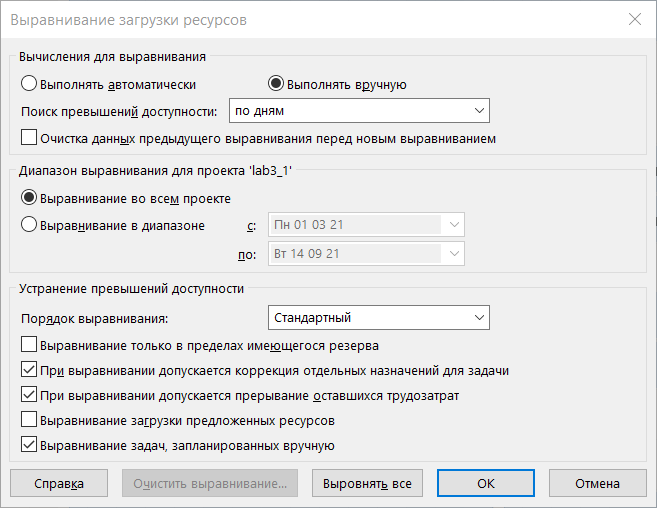
\includegraphics[width=0.7\linewidth]{src/lab3_1_1}
	\caption{Выравнивание}
	\label{fig:lab311}
\end{figure}

В результате выравнивания перегрузка ресурсов была устранена.










